\documentclass[14pt,a4paper]{article}
\usepackage{txfonts}
\usepackage[utf8]{inputenc}
\usepackage[spanish]{babel}
\usepackage{amsmath}
\usepackage{amsfonts}
\usepackage{amssymb}
\usepackage{makeidx}
\usepackage{graphicx}
\usepackage{lmodern}
\usepackage{kpfonts}
\usepackage{fourier}
\usepackage{natbib}
\usepackage[left=2cm,right=2cm,top=2cm,bottom=2cm]{geometry}
\author{Rodriguez Lopez Francisco Javier}


\begin{document}
\begin{center}
\paragraph{\large UNIVERSIDAD POLITECNICA DE LA ZONA METROPOLITANA DE GUADALAJARA}


\includegraphics[width=6cm]{Upzmg.png} 
\end{center}
\begin{center}
\textbf{\LARGE Segundo Avance}\\
\end{center}
\begin{center}
\textbf{\LARGE Brazo Robotico}
\end{center}


\large{Integrantes:}\\
\begin{itemize}
\large{\item Cabrera Gutierrez Raul.
\item Gutierrez Olivares Rogelio.
\item Guzman Vazquez Jaime Alan Yamil.
\item Perez de Alba Santiago Eduardo.
\item Rodriguez Lopez Francisco Javier.
\item Romero Jauregui Osvaldo.
\end{itemize}


Fecha: 23 de octubre del 2019.\\

Curso: Sep-Dic 2019.\\

Carrera: Ingenieria en Mecaronica.\\

Docentes:\\
Moran Garabito Carlos Enrique.\\
Vazquez Alcaraz Laura Eugenia.}

\newpage

\section{Titulo de Proyecto:}

Brazo robotico multidiplicinario con acoplamiento para diferentes tareas de grado industrial con gran libertad de movimiento y solucion de problemas industriales.


\section{Planteamiento del problema:}

Para poner cierto contexto en este proyecto se presentaran las diferentes cuestiones que orientan a la realizaciòn de este proyecto  por diferentes cuestiones, los brazos robòticos son ùtiles y en el ambito empresarial, estos son muy utilizados por su versatilidad y fàcil programaciòn.\\
El brazo robòtico tiene gran importancia en la industria, en general por esto se alento a la realizaciòn de este, debido a que tienen gran potencial y puede ser maniobrado en diferentes àmbitos debido a su disposiciòn y versatilidad.\\
Las dificultades de este proyecto a futuro podrìan ser cuestiones como el presupuesto, este serìa una de las mayor dificultades, a esto se le suman cuestiones como la cotizaciòn de todos los materiales y precios para conseguir las mejores ofertas asì como los componentes.\\
Otra de las dificultades podria ser la compatibilidad con los diferentes accesorios para las que serìa utilizado este brazo, debido a que 
este tipo de automata es empleado para las diferentes cuestiones de la industria.\\
Estas dificultades son de gran importancia para este proyecto, debido a que en cuestiòn de presupuesto o de inversiòn este proyecto necesita piezas relativamente costosas ya que se necesitan componentes de calidad para garantizar la cuestiòn de la durabilidad.\\
Para las dificultades anteriores se propone las distintas soluciones para la cuestiòn del presupuesto. La soluciòn a esto serìa abaratar costos creando la base de el brazo de materiales reciclados o materiales economicos. Ademàs de tener una planificaciòn en cuestiòn del presupuesto con un ingreso a plazos, el proyecto esta basado a un año y la mejor forma de administrar este proyecto serìa un buen uso de los componenetes ya que la perdida de alguno de estos podria ocacionar un gasto innesesario, esto podrìa solventar el problema de el presupuesto.\\
Para resolver el problema de la compatibilidad con las piezas de otros fabricantes, se implementara un sistema de intercambio de cabezales para lograr que el brazo robòtico pueda ser compatible con estas diferentes piezas, ademàs de generar acoplamientos o adaptadores para el brazo robòtico. \\
Las diferencias que se encuentran en el campo industrial con este proyecto, es que el proyecto es completamente echo con componentes comerciales, mientras que los brazos robòticos industriales estàn generados a mucho mayor costo ademàs de componentes de grado industrial, de mayor durabilidad y calidad, sin embargo este proyecto puede ser tomado como prototipo pero podrìa ser llevado a gran escala.\\
El sustento en el que se basan los datos anteriores seria basado en el mercado actual, asì como los datos obtenidos del mercado al igual que el funcionamiento de estos y los componentes utilizados asì como su precio en diferentes tiendas, asì como en linea.\\
Los puntos anteriores esta basados en conocimientos adquiridos mediante el estudio de la implementaciòn en los medios industriales, al igual que su funcionamiento.

\section{Formulacion de Problema:}

En este apartado, se estaran viendo las preguntas que se puedan generar respecto a un futuro, dentro del proyecto:\\

¿Es buena idea suplementar este tipo de dispositivos para otras actividades ademàs del personal humano?\\
¿El brazo es algo eficiente a la hora de realizar su tarea?\\
¿Se puede, implemetar para tareas complejas que sean de eficiencia y ràpidez?\\
¿Es buena idea de la implementaciòn de la automatizaciòn con este tipo de dispositivos? 

\section{Objetivo General:}

Creacion de un brazo robòtico con la finalidad de adaptacion a tareas complejas que el personal humano no realice con exactitud, mediante los conocimientos adquiridos y la demostracion de habilidades y aptitudes que se tengan. 

\section{Objetivos del Proyecto:}

\begin{itemize}
\item Analizar y describir el buen funcionamiento del brazo robòtico.
\item Empleamiento de tareas de atomatizaciòn.
\item Diseñar un modelo eficiente que capacite y proponga formas de adaptaciòn a tareas humanas.
\item Demostrar los conocimientos que se adquieran, en los cursos. 
\end{itemize}

\section{Justificacion:}

El brazo robòtico, es una herramienta eficiente para ambientes, insutria-empresariales, para funciòn y mejora del trabajo del personal comùn, que mejora la ràpidez, fluidez y sustenciòn del trabajo a realizar o en este caso alguna tarea en particular. El brazo robòtico suplementa en eficiencia las tareas del humano, al fin de remplazar la lentitud y errores que este tiene.\\
El proyecto planteado en sintesis, tiene como idea, el  poder suplementar esas tareas empresariales que cuesta mucho dinero, energìa y trabajo en cuestiòn, tratando complejos casos como la falta de personal, siendo este la sustituciòn perfecta para las manos laborales ordinarias, ambientado en el sector de automatizaciòn y robòtica, el cual pueda tambièn agarrar temas, de control, y sustentaciòn de las herramientas que se utilizaràn en este proyecto, que en relevancia se adapte tanto al equipo como conocimiento, a la sociedad una herramienta que pueda ser mejor innovada y utilizada, en otros campos.\\
Estructurado en primera instancia a la industria, la mecatrònica y sus amplias gamas de estudio que puede cubrir para la mejoraciòn e implentaciòn, en las tareas que este pueda realizar, siendo varias y de ello, poder visulalizar en que constancia este dispositivo este apto para temas de mayor complejidad, viendo las problemàticas que este tiene, a la  hora de implementarlos el sector de automatizaciòn, y las ganancias mismas de este.

\section{Limitacion:}
Las limitaciones mas evidentes que podria tener este proyecto podrian ser cuestiones como el lìmite de peso que podrìa cargar, puesto que los materiales, los componentes asì como la estructura general de este, va estar diseñada para contener cierta capacidad de carga que seria en un rango entre los 400 g y los 700 g, limitandose a està, reiterando debido a cuestiones bàsicas de presupuesto ademàs de conocimientos debido a que estamos en un ciclo de formaciòn intermedio durante la ingenierìa que lìmita el uso de algunas herramientas que màs tarde se ven planeadas a ser utilizadas, puesto que este proyecto sera retomado para el ùltimo ciclo de formaciòn en donde se actualizaran materiales y estructuras, asì como componentes para mejorarlo, abundando en esto otra de las limitantes que podria ser el precio de los componentes en general ya que es bien sabido que a mayor calidad mayor son los costos involucrados en la elaboraciòn de estè, puesto al tamaño del proyecto asi como las restricciones econòmicas que se tienen, esto lìmita tambièn el proyecto,\\
Las dimensiones de estè tambièn podrian ser una limitante, ya que por supuesto limitan la cantidad de peso que puede ser soportado, asì como la maniobrabilidad de estè, asì como variables como la resistencia de materiales puede afectar a este brazo.\\
Otras cuestiones que tambièn lìmitan de forma grande al proyecto podrian ser la cuestiòn de base a la que se cuenta, es decìr el propòsito al que se quiere llegar y como esto cierra el camino hacia otras posibilidades, se obtara por hacer este proyecto lo mas universal por asì decirlo que se pueda, que se pueda utilizar en diferentes àmbitos sin que su contrucciòn pueda ser una limitante. Sin embargo habra cosas que no pueda hacer a menos de que se restructure todo el mecanismo y materiales  de estè, un ejemplo de esto podrìa ser el enviarlo a lugares con bajas temperaturas o con grandes dificultades de movimiento, para lo que no fue diseñado.

\section{Delimitacion:}

Las delimitaciones en las que nos enfocaremos, seran en mayor parte la eficiencia del brazo robòtico, a la hora de mostrar el funcionamiento de estè.\\
El àrea a centrarse, a partir de dicho planteamiento, y limitantes, es en la especificaciòn de los grados de libertad que este brazo pueda tener, àdemas de cuanto es el peso que este pueda sostener, y por cuanto tiempo puede hacerlo, optimizando el trabajo mecànico que realizaria dicho dispositivo, a fin de centrarnos en otros temas, como la velocidad en que realiza dichas tareas, asi como la complejidad o la fluidez en las que hace realiza dichas tareas.\\
Al fin de ver las fronteras de espacio-tiempo, que el estudio pueda tener. En secciones muestrales en donde se especìfica de mejor forma cada elemento a estudiar y a delimitar, en cierta parte, desde el tema del peso, hasta el tema de cuanto es el alcance que este brazo pueda alcanzar, esto viendolo a muestreo, y en rasgos de prueba , dureza, firmeza, y càlculos fìsicos, el cual a partir de la dinàmica del dispositivo, se puedan demostrar las areas a  mejoras y limitantes en la conceptualizaciòn de lo que es el brazo robòtico, siendo este una temàtica que se realizarìa dentro del desarrollo del brazo y su anàlisis de estudio,

\section{Marco Teorico:}

\subsection{Robots:}
Robots are diverse bunch. Som walk around on their two, four, sic or more legs, while others can take to the skies. Som robots help physcian to do surgery inside your body; others toil away dirty factories. There are robots the size of a coin and robots bigger than a car. Some robots can make pancakes. Others can land on Mars.

\subsection{Robot Arm:} 
A robot arm is a type of robot consisting of parts linked together in the same way as those of a human arm, monted on a stand.
The most common manufacturing robot is the robot arm which is usually made up of several metal segments.
Sensors were fixed to the robot arm to detect whether there were humans close to the robot.
A robot arm is a type of robot consisting of parts linked together in the same way those of a human arm, mounted on stand \citep{schilling1990fundamentals} .


\newpage

\section{Desarrollo:}

\section{Aportacion a cada Materia:}

\begin{tabular}{|p{70mm}|p{70mm}|} 

\hline
	MATERIAS & APORTACIONES ESPERADAS\\
\hline
	INGLES & La materia de ingles es importante puesto que toda la programacion se realizara en ingles al igual que las fuentes de informacion consultadas.\\
\hline
	SISTEMAS ELECTRONICOS DE INTERFAZ & Esta materia ayudara a generar los conocimientos para realizar la fuente de voltaje que necesita el proyecto\\
\hline
	PROGRAMACION DE PERIFERICOS & Los conocimientos de la programacion del brazo se originan de esta materia.\\
\hline
	CONTROLADORES LOGICOS PROGRAMABLES & La aportacion de esta materia seria el grafcet para la  programacion del proyecto\\
\hline
	ESTRUCTURA Y PROPIEDADES DE LOS MATERIALES & normas de seguridad como seleccion de materiales para estructura\\
\hline
	ETICA PROFESIONAL & responsabilidad y seguimiento de normas al momento de realizar las evidencias del proyecto ademas  de dar seguimiento a los còdigos establecidos para la ingenierìa.\\
\hline
\end{tabular}\\\\


\begin{tabular}{|p{70mm}|p{70mm}|} 

\hline
	MATERIAS & APORTACIONES REALIZADAS\\
\hline
	INGLES & Se consultaron fuentes de informaciòn en inglès para la realizaciòn de los circuìtos y programaciòn.\\
\hline
	SISTEMAS ELECTRONICOS DE INTERFAZ & Se aplican los diferentes componentes vistos en la materia para realizar la fuente de voltaje variable.\\
\hline
	PROGRAMACION DE PERIFERICOS & Se utiliza phyton y su generaciòn de interfaz para el control del brazo.\\
\hline
	CONTROLADORES LOGICOS PROGRAMABLES & Se diseña el grafcet para la mejor estructuraciòn de la programaciòn.\\
\hline
	ESTRUCTURA Y PROPIEDADES DE LOS MATERIALES & Se investigan los diferentes posibles materiales para la estructura del proyecto de acuerdo a sus propiedades.  \\
\hline
	ETICA PROFESIONAL & Se siguen los comportamientos eticos durante el proceso de realizacion del proyecto como podria ser la autonomia del profesionista, ademas de atender al codigo profesional de ingenierias.  \\
\hline
\end{tabular}


\section{Diagramas:}

\begin{center}
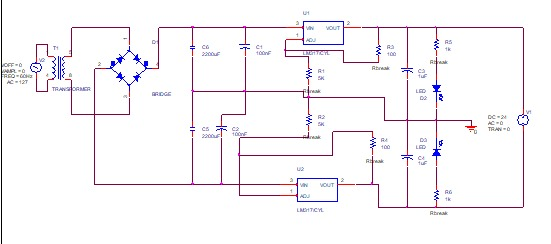
\includegraphics[width=12cm]{Fuente.jpeg} 
\end{center}

En el diagrama de la fuente de alimentaciòn regulada, se pueden ver los componentes que esta tendra, siendo el màs destacado de ello el regulador de voltaje lineal Lm317, se propuso este componente, como una estimaciòn de lo que otros componentes podrìan tambièn hacer, como lo es regular el voltaje y variarlo al valor que se mecesite (En este caso para los motores), pero esto lo estimaremos mejor ya que entremos a temas de convertidores de voltaje, en la clase de Sistemas Electrònicos de Interfaz. Por esta parte adquiriendo el conocimiento suficiente para poder establecer un mejor componente, o un mejor acomodo del esquemàtico,para mejoras e innovaciones que podria tener el sintetizar este tipo de fuentes para el uso en el trabajo mecànico, en cuestiòn de potencia. En este se toma en cuenta que el voltaje mìnimo que puede manejar son 1,25v a 100mA, especificaciones que son de ayuda.\\

Nota: En la parte, de la transformaciòn, se encuentra un panel de amperimetro/voltimetro, el cual no fue añadido a vista, dadas las faltas del saber del software, àdemas de la realizaciòn de regulaciòn (Que puede ser modificada, al tener mejor y mas apto conocimiento).

\section{Calculos:}
En secciòn al càlculo del brazo robòtico. Para poder empezar con el càlculo dinámico de este brazo robòtico, en constancia de previsualizaciòn a una estimaciòn dada hipotesis en perpectiva a los materiales y a la resistencia que tendran estos, para el movimiento, carga y distribuciòn de peso de este, Siendo estè caso, màs simplificado, para no atraer problemas a la hora del armado que tenga estè y sus piezas.\\

Caracterìsticas del brazo:\\
Altura: 40 cm apoximadamente.\\
Peso: 8Kg aproximadamente.\\
Caracterìsticas del motor:\\
Voltaje dc: 6v-24v.\\
Corriente: 1.10 A.\\
Revoluciones: 10,000rpm.\\
Diametro del motor: 36mm.\\
Diametro del torque: 3.17mm.\\
Con esas caracterìsticas, se puede dar una idea, de como quedarìa establecida la dinàmica del brazo robòtico, en este caso, viendo màs que nada factores como los motores, o el peso que cargara el brazo y en estancìa con que esfuerzo.\\
Se càlcula de primera estancìa el trabajo de los motores, estabeciendo el trabajo de estos:\\

Establecemos el punto de partida de la posiciòn en la que se encontara al momento del giro del motor:\\

$$ \emptyset=\frac{4mm}{3.17mm}= 1.3mm $$

En constancia al centro del diametro, el momento en que se mueve este, se encontrara en 1.3mm, respectivamente en movimiento.\\
Ahora queremos cambiar de revoluciones, a radianes por segundo, para asi poder ver el movimiento en los 360°, que esta establecido el torque del motor, quedando:\\

$$ 1rev=2\pi=360°$$

$$ 10,000 \frac{vueltas}{min}*\dfrac{2\pi rad}{1 vuelta}*\frac{1 min}{60s}= 333.3 \pi rad/s $$

Simplificando \pi queda:\\

$$ 333.3 rd/s* \pi= 1,047.2 rd/s $$

Ahora teniendo datos, simplificados, para ver como trabajara en la realizacion mecanica, el motor, podremos calcular el momento, entre otros factores del brazo, para su péso en una previsualizacion.\\

$$ M= P*D $$

Simplificando datos:\\

$$ M=0.40m*8kg= 3.2 m/kg $$

Esto ayuda a la hora de carga del objeto en cuanto la garra, y el motor, simplificando el trabajo que pueda hacer tanto mecanico, como de potencia.\\
En otro punto, el centro de masas nos ayuda en este caso, a ver el estable movimiento en el que se puedan encontrar tanto el peso del brazo, como el del objeto a cargar, siendo este:\\

$$ CM=\frac{3.2 m/kg}{8kg}= 0.40m $$

Como se aprecia en el resultado, nos da el inicio del brazo, esto quiere decir que el centro de estabilidad, se encuentra al principio de este. Conceptuando la longitud que tendra el brazo, y donde tendra todo su impetu, a la hora de carga y de trabajo.\\
En otro caso, el trabajo que pueda realizar este, dejandolo con la siguiente formula:\\

$$ W= F*cos(45°)*d $$

Esta formula respectivamente del angulo es un alcance del angulo que puede tener para la liberacion de grados de libertad.\\

$$ W= 160N*cos(45°)*0.40m= 48.7 J $$

Dejandonos apreciar el trabajo que podriamos tener, en un punto del agarre.\\

Nota: Estos calculos, solo son una perpectiva, de lo que podria ayudarnos, a terminos mas complejos, como el caso de las articulaciones, y el manejo de la potencia en conjunto, siendo estos una guia de poder ver la realizacion y el armado, de los motores respecto al centro de carga y el alcance que podria tener, este brazo robotico, analizandolo mas adelante, con dinamica avanzada.\\

\textbf{Fuente de Alimentacion Variable:\\}
Los calculos de la fuente variable queda establecido en la visualizacion del esquematico:\\
La formula para la obtencion del voltaje, dadas resietncias es:\\
$$ V_{out}= 1.25v(1+\frac{R1}{R2}) $$
Obteniendo datos:\\
$$ V_{out}= 1.25v(1+\frac{3900 ohm}{220 ohm})=23.4 voltios $$
Esta primera formula sintetiza, los valores de la resietncia R1 y R2, que nos ayudan a que el flujo de la corriente sea especifico. Quedando el voltaje de salida en 23.4v.\\

$$ Vp= \frac{V_{rms}}{0.707} $$

Obteniendo datos:\\

$$ Vp=\frac{16v}{0.707}= 22.6 v $$

Esta formula obtiene los datos, del Vrms, los 16v, son los del transformador que se podria utilizar. Ahora se aprecia en el esquematico, que hay un puente de diodos, conectando dos diodos, al transfromador y los otros tanto parte negativa, como parte posityiva del Lm317 en el Vin, nos dejan un resultado de la asiguiente forma:\\

$$ V_{dc}=\frac{2(22.6v)-1.4v}{\pi}= 14 v. $$

En este calculo, se tiene en cuenta que son dos diodos los que estan trabajando sobre la misma entrada, por lo que un solo diodo tiene 0.7v, esto multiplicado por dos seria 1.4v. En otro caso el dos que mutiplica al voltaje 22.6, es la cantidad de diodos que hay en ese punto.\\
Teniendo ya los voltajes, se saca la potencia con la que trabajaremos, en este caso, entre mas potencia haya, menos ruido podra tener la regulacion del voltaje, en este caso, siendo multiplicado por dos el voltaje del transformador, nos da un resultado de 32 Vatios. Ahora si sacamos la corriente establecida en el diagrama.\\

$$ P= (V)(I)= 32vatios=(22.6v)(I) $$

Sustituyendo la formula, para encontrar la corriente se hace un despeje:\\

$$ I= \frac{32va}{22.6v}= 1.4 A $$

Este valor de corriente, establecida en todo el circuito es la indicada, para el buen torque de los motores, y el movimiento de estos.\\
Para el uso de los capacitores es bueno tener en cuenta de que valor y de que capacidad se tendran que tener, pqara establecer un mejor flujo del voltaje. En los primeros dos capacitores son electroliticos, con un valor en Faradios de 2200uF a una capacidad de 30v, esto para que el voltaje que recae en las resistencias sea bien distribuido y no se sobrecargue el condensador.\\
Los segundos, son ceramicos, esto para que el flujo de corriente y el momento de carga sea mas pura, con un valor de 100nF a una capacidad de 50v, para que administre de mejor forma la regulacion de voltaje y la tercera linea de capacitores es de 1uF a 30v, esto para lo mismo, que al momento de carga, no se desperdicie demasiado, y pueda salir el voltaje que se requiere, para el funcionamiento correcto de los motores.

\section{Diagrama de Gantt posibles Materiales y Gastos:}

\begin{center}
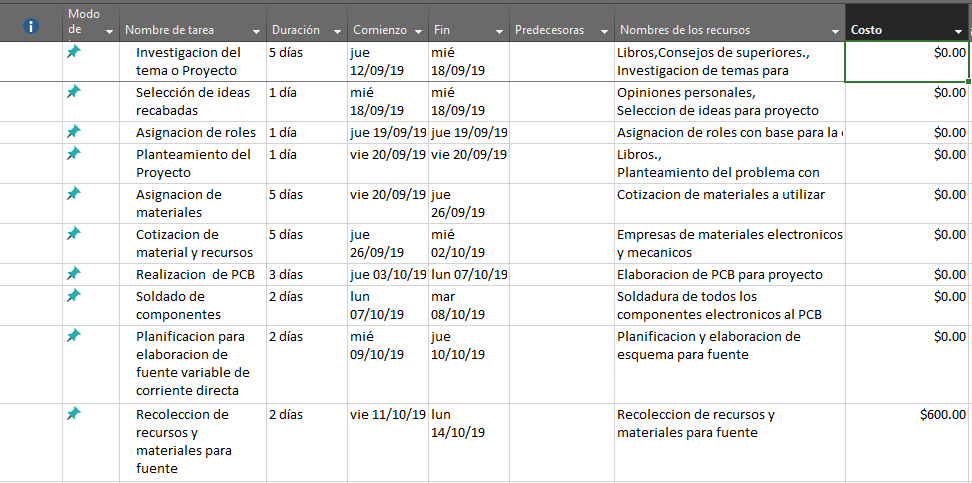
\includegraphics[width=15cm]{DefinicionTareas/4.png} 
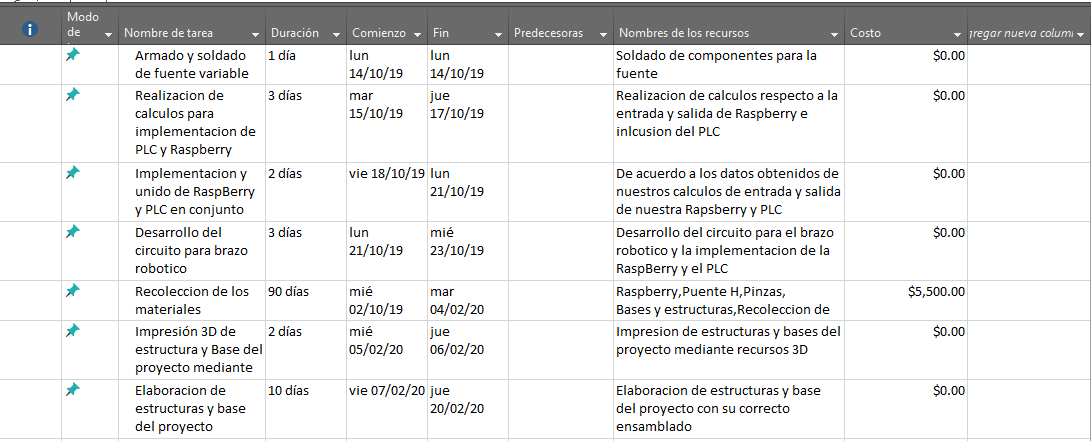
\includegraphics[width=15cm]{DefinicionTareas/5.png} 
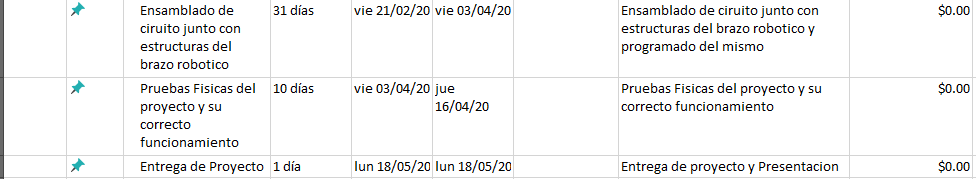
\includegraphics[width=15cm]{DefinicionTareas/6.png} 
\end{center}

\newpage
\section{Diagrama de Gantt Cronograma de Actividades y Tiempo:}
Cronograma de trabajo, fechas establecidas del 12 de  Septiembre del 2019 al dia de entrega, 18 de mayo del 2020

\begin{center}

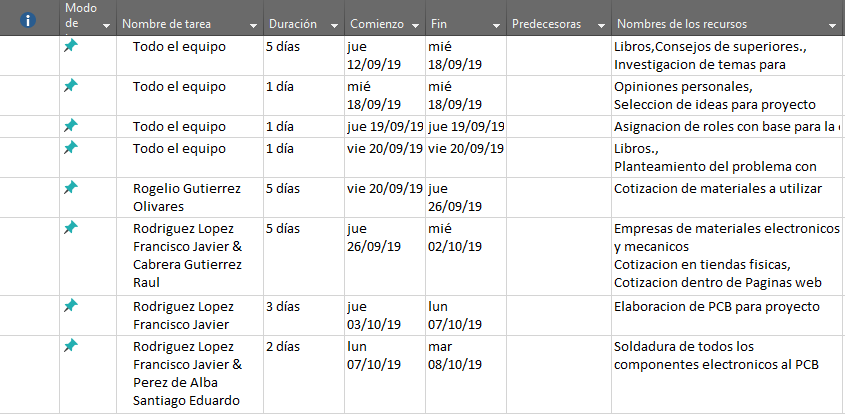
\includegraphics[width=13cm]{Esquema1.png} 
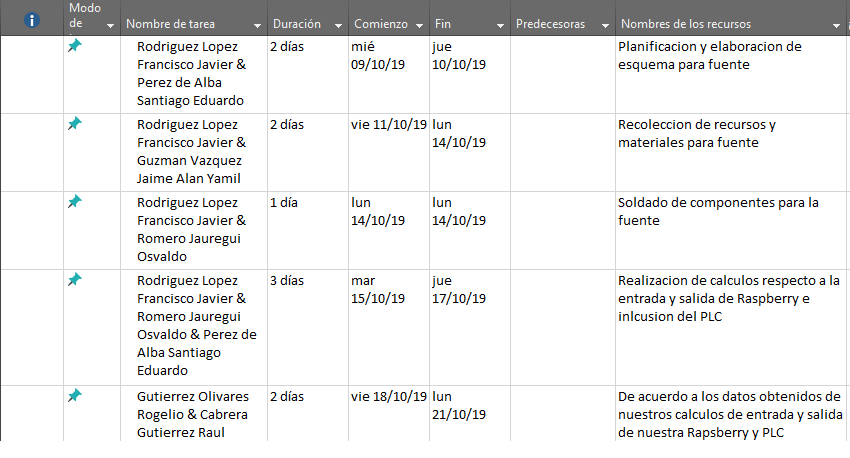
\includegraphics[width=13cm]{Esquema2.png} 
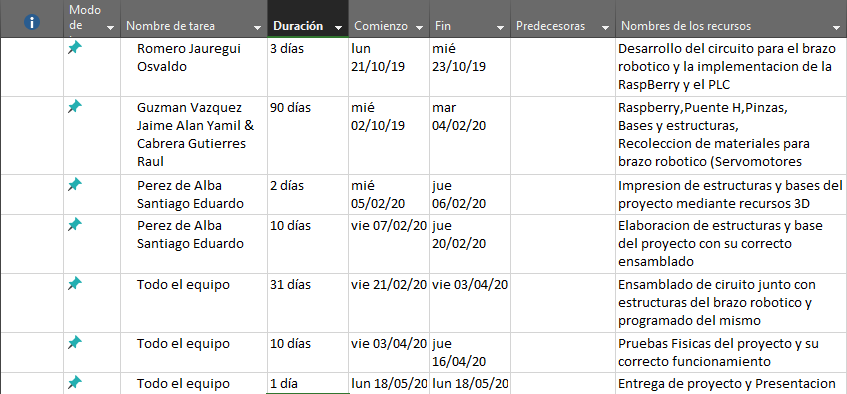
\includegraphics[width=13cm]{Esquema3.png} 

\end{center}

\section{Propuesta de Materiales:}

\subsection{Elementos consturctivos}
\begin{enumerate}
\item Manipulador o brazo mecanico.
\item Elementos motrices o actuadores.
\item Controlador.
\item Efector terminal.
\item Sensores de informacion.
\item Motor a Pasos.
\end{enumerate}

\subsection{Manipulador}
Es el conjunto de elementos mecanicos que permiten el movimiento del efector termina. En la estructura interna del manipulador se encuentran ubicador muchas veces los elementos motrices, engranajes y tranmisiones que soportan el movimiento de las cuatro partes, que por lo geneal conforman el manipulador, las cuales son \citep{puglisi2006protesis}:\\
1-Base o pedestal de fijacion.\\
2-Cuerpo.\\
3-Brazo.\\
4-Antebrazo.\\
\subsection{Elementos motrices o Actuadores}

\begin{itemize}
\item \textbf{Neumaticos}:
Emplean aire comprimido como fuente de energia y son adecuados en el control de movimientos rapidos, pero su precision es limitada.\\
\item \textbf{Hidraulicos}:
Los actuadores hidraulicos son recomendables en los manipuladores que tiene una gran capacidad de carga, junto a una precisa regulacion de velocidad \citep{turiel2002aplicaciones} .\\
\item \textbf{Electricos}:
Los motores electricos son los mas utilizados, gracias a su precision y la facilidad de control.
\end{itemize}

\subsection{Controlador:}
Es el dispositivo encargado de regular el movimiento de todos los elementos del manipulador, y de realizar los calculos y procesado de la informacion. La complejidad del control varia segun los pramatros que se gobiernan \citep{cardenas2015diseno}.
\subsection{Efector Terminal:}
Es la garra o herramienta que se le acopla a la muneca del manipulador, siendo el encargado de materializar el trabajo previsto por ejemplo, este puede ser una tenaza, un electroiman, o algun otro aparato. En general, y de acuerdo al tipo de aplicacion, la problematica del efector terminal radica en que este ha de posser una elevada capacidad de carga y al mismo tiempo es importante que tenga un peso y tamano reducido. Por esto, en muchas ocasiones es necesario disenar el efector terminal de acuerdo a los requerimientos de la aplicacion en que se utilizara.
\subsection{Sensores de Informacion:}
Los robot inteligentes son aquellos capaces e adaptarse al ambiente y tomar decisiones en tiempo real, adecuadas para situacion. La informacion que ellos reciben les hace autoprogramables, es decir,alteran su actuar en funcion de la situacion externa, lo que los hace poseer un cierto grado de inteligencia artificial. A este respecto, las informaciones mas solicitadas por los robots son las que hacen referencia a la posicion, velocidad, aceleracion, fuerzas,pares, dimensiones y contornos de objetos, y temperatura.
\subsection{Motor a Pasos:}
\textbf{Funcionamiento:}\\
Este motor a pasos NEMA17 es bipolar, tiene un angulo de paso de 1.8°(200 pasos por vuelta) y cada bobina es de 1.2A a 4V, capaz de cargar con 3.2kg/cm. Es un motor muy robusto ampliamente utilzado en impresoras 3D caseras.
\textbf{Caracteristicas:}\\
Este motor cuenta con:\\
\begin{enumerate}
\item Tamano: 42.3*48mm, sin incluir el eje.
\item Peso: 350 gramos.
\item Diametro del eje: 5mm.
\item Longitud del eje: 25mm.
\item Pasos: 200.
\item Corriente: 1.2 Amperios por bobinado.
\item Tension: 4V.
\item Resistenica: 3.3 Ohm por bobina.
\item Torque: 3.2kg/cm.
\item Inductancia: 2.8 mH por bobina.
\end{enumerate}
\textbf{Aplicacion:}\\
Los motores paso a paso se utilizan generalmente en una variedad de aplicaciones donde el control de posicion exacra es deseable y el coste o la complejidad del sistema de control sea justificada.\\
\begin{enumerate}
\item Impresoras CNC.
\item Impresora 3D / prototipos de maquinas.
\item Cortadoras laser.
\item Actuadores lineales.
\item Discos duros .
\end{enumerate}

\section{Presupuesto:}

\begin{tabular}{|l|l|l|l|}
\hline
	Producto & Piezas & Precio & Total\\
\hline
	Impresion 3D & 5 & 70 & 350\\

\hline
	Capacitores 2200uF,1uF, 100nF & 3 & 5 & 15\\
\hline
	Regulador LM317 & 1 & 15 & 15\\
\hline
	Resistencias varias & 20 & 2 & 40\\
\hline
	Diodos1N4004G & 16 & 5 & 80\\
\hline
	1 Switch & 1 & 10 & 10\\

\hline
	Fuente CA-CD & 1 & 600 & 600\\
\hline
	Push bottons & 8 & 2 & 16\\
\hline
    Cautin & 1 & 150 & 150\\
\hline
	Estaño & 1 & 30 & 30\\
\hline
	Multimetro & 1 & 100 & 100\\
\hline
    Motores DC & 5 & 400 & 2000\\
\hline
\end{tabular}

\section{Prototipo y Simulacion:}
\begin{center}
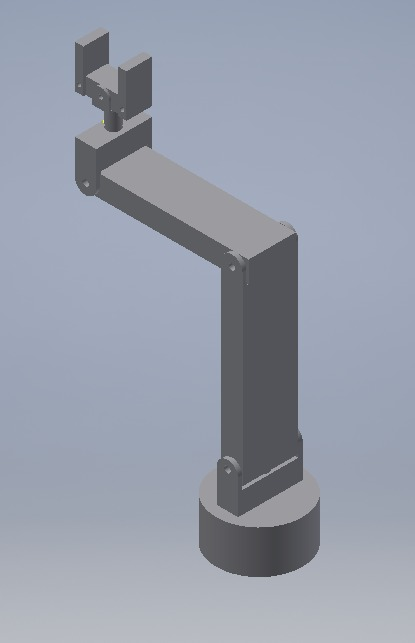
\includegraphics[width=6cm]{Proto.jpeg}
\end{center}

\newpage

\bibliographystyle{plain}
\bibliography{Ref}


\end{document}